\documentclass[conference]{IEEEtran}

\usepackage{amsmath}
\usepackage{amssymb}
\usepackage{graphicx}
\usepackage{booktabs}
\usepackage{multirow}
\usepackage{url}
\usepackage{cite}
\usepackage{xcolor}
\usepackage{tabularx}
\usepackage{array}
\usepackage{makecell}

\begin{document}

\title{Avian Influenza Genomic Intelligence: A Hybrid Deep Learning Architecture for Pathogenicity Category Prediction and Mutation-Aware Sequence Modeling}

\author{
    \IEEEauthorblockN{Vishnu Varthan Senthilkumar}
    \IEEEauthorblockA{\textit{Department of Artificial Intelligence and Data Science} \\
    \textit{Genomic Intelligence Framework Project} \\
    Email: vishnuvarthan63@gmail.com}
}

\maketitle

\begin{abstract}
High-consequence avian influenza viruses, such as H5N1, H5N8, and H7N9, have led to mass poultry mortality, severe economic losses in agriculture, and confirmed human deaths across several continents, highlighting a major inadequacy in pandemic preparedness infrastructure. The traditional wet-lab approach of pathotype characterization by in vivo inoculation assays and serological profiling at high containment levels is not scalable to meet the throughput needs of genomic epidemiology based on next-generation sequencing. To overcome this surveillance limitation, we introduce the Avian Influenza Genomic Intelligence Framework, an integrated hybrid multimodal deep-learning system comprising 10.30 million trainable parameters for real-time viral nucleotide sequence pathotype stratification across four epidemiologically based risk strata: Avirulent, Low Pathogenicity, Moderate-High Pathogenicity, and Highly Pathogenic. The architecture couples a DNABERT-2-inspired transformer encoder capturing local hexamer contextual representations with a HyenaDNA-inspired sub-quadratic long-convolution module modeling long-range dependencies. A reference-guided mutation prioritization engine extracts, biologically scores, and encodes alignment mismatch loci into a structured variant feature tensor. An eight-head cross-attention fusion layer dynamically routes virulence mutation queries across the joint dual-stream sequence context, enabling targeted variant-aware feature integration. Trained on a curated NCBI-derived benchmark of 35,211 sequences across 72 FASTA files and evaluated on a stratified hold-out test set of 6,691 sequences, the framework achieves an overall accuracy of 98.03\%, macro ROC-AUC of 96.47\%, weighted F1-score of 97.89\%, and Matthews Correlation Coefficient of 0.8921, with an average inference latency of 12.82~ms per sequence. Gradient-based explainability analysis demonstrates that classification decisions are rooted in biologically relevant genomic regions, establishing the system as a scalable, interpretable tool for pandemic-era avian influenza biosurveillance.
\end{abstract}

\begin{IEEEkeywords}
Avian Influenza Biosurveillance, Viral Pathotype Stratification, Hybrid Deep Learning, Cross-Attention Fusion, Explainable Genomic Intelligence.
\end{IEEEkeywords}

\section{Introduction}
\label{sec:introduction}

Avian influenza A viruses (AIV) present continuous global public health challenges due to cross-species transmission events, poultry flock mortalities, and agricultural disruptions~\cite{who2024avianflu, naeem2022hpai}. Highly Pathogenic Avian Influenza (HPAI) strains, notably within the H5 and H7 subtypes, often induce severe systemic infection in gallinaceous poultry and have caused documented human infections with case-fatality rates exceeding 50\%~\cite{subbarao1998h5n1, cheung2007pathogenicity, soda2022influenza}. In contrast, Low Pathogenic Avian Influenza (LPAI) strains (such as H9N2, H5N2, and H7N2) circulate widely in wild aquatic bird reservoirs, where they can acquire point mutations at the hemagglutinin (HA) cleavage site, receptor-binding pocket, or polymerase subunits (PB2/PA) that facilitate rapid conversion to high pathogenicity~\cite{influenza2010pandemic}.

Standard diagnostic classification relies on laboratory determination of the Intravenous Pathogenicity Index (IVPI) in specific-pathogen-free (SPF) chickens, supplemented by Sanger sequencing of the HA proteolytic cleavage motif~\cite{soda2022influenza}. While biologically definitive, these wet-lab protocols demand Biosafety Level 3 (BSL-3) containment, require multi-day turnaround periods, and cannot scale to high-throughput genomic surveillance networks processing next-generation sequencing (NGS) data in real time~\cite{libbrecht2015ml}.

Recent progress in biological language modeling has shown that deep neural networks can extract informative representations directly from nucleotide sequences~\cite{ji2021dnabert, zhou2023dnabert2, nguyen2023hyenadna}. Transformer architectures such as DNABERT~\cite{ji2021dnabert} and DNABERT-2~\cite{zhou2023dnabert2} employ bidirectional self-attention to learn contextual representations of overlapping $k$-mer tokens. However, standard self-attention exhibits quadratic complexity $\mathcal{O}(L^2)$ with respect to sequence length $L$, which limits scalability on long viral contigs without aggressive chunking~\cite{vaswani2017attention, chen2020bigbird}. Conversely, sub-quadratic operator hierarchies, such as HyenaDNA~\cite{nguyen2023hyenadna} and structured state-space models~\cite{gu2021mamba, poli2023hyena}, model long-range dependencies at single-nucleotide resolution using long causal convolutions and data-controlled gating.

Although sequence-level encoders capture broad contextual patterns, viral pathogenicity is frequently governed by discrete, highly localized point variations (e.g., polybasic insertions at the HA cleavage site). Standard sequence-only models often fail to explicitly isolate, score, and integrate these specific mismatch loci relative to reference viral genomes.

To address this challenge, we present the \textbf{Avian Influenza Genomic Intelligence System}, a hybrid deep learning architecture designed for automated, mutation-aware pathogenicity classification. Our contributions are summarized as follows:
\begin{enumerate}
    \item \textbf{Dual-Stream Sequence Representation}: We combine a 4-layer DNABERT-2-inspired transformer ($k=6$, vocabulary size 4,096) for localized $k$-mer representation with a 4-layer HyenaDNA-inspired long-convolution module to capture both local sequence motifs and extended structural context.
    \item \textbf{Reference Alignment and Mutation Encoding}: We develop an automated bioinformatic module that validates sequence quality, standardizes sequence length, extracts mismatch loci relative to reference sequences, scores variations via regional and spatial heuristics, and encodes the top-32 mutations into a dense numerical tensor.
    \item \textbf{Cross-Attention Multi-Modal Fusion}: We implement an 8-head cross-attention mechanism where prioritised mutation query vectors interact with the joint sequence context, followed by global average pooling and an MLP classification head.
    \item \textbf{Rigorous Empirical Characterization}: We provide an exact layer-by-layer parameter profile (10,303,748 trainable parameters), evaluate hold-out performance on 6,691 test sequences across 4 curated pathogenicity categories, and provide gradient-based attribution analysis.
\end{enumerate}

\begin{figure*}[t]
    \centering
    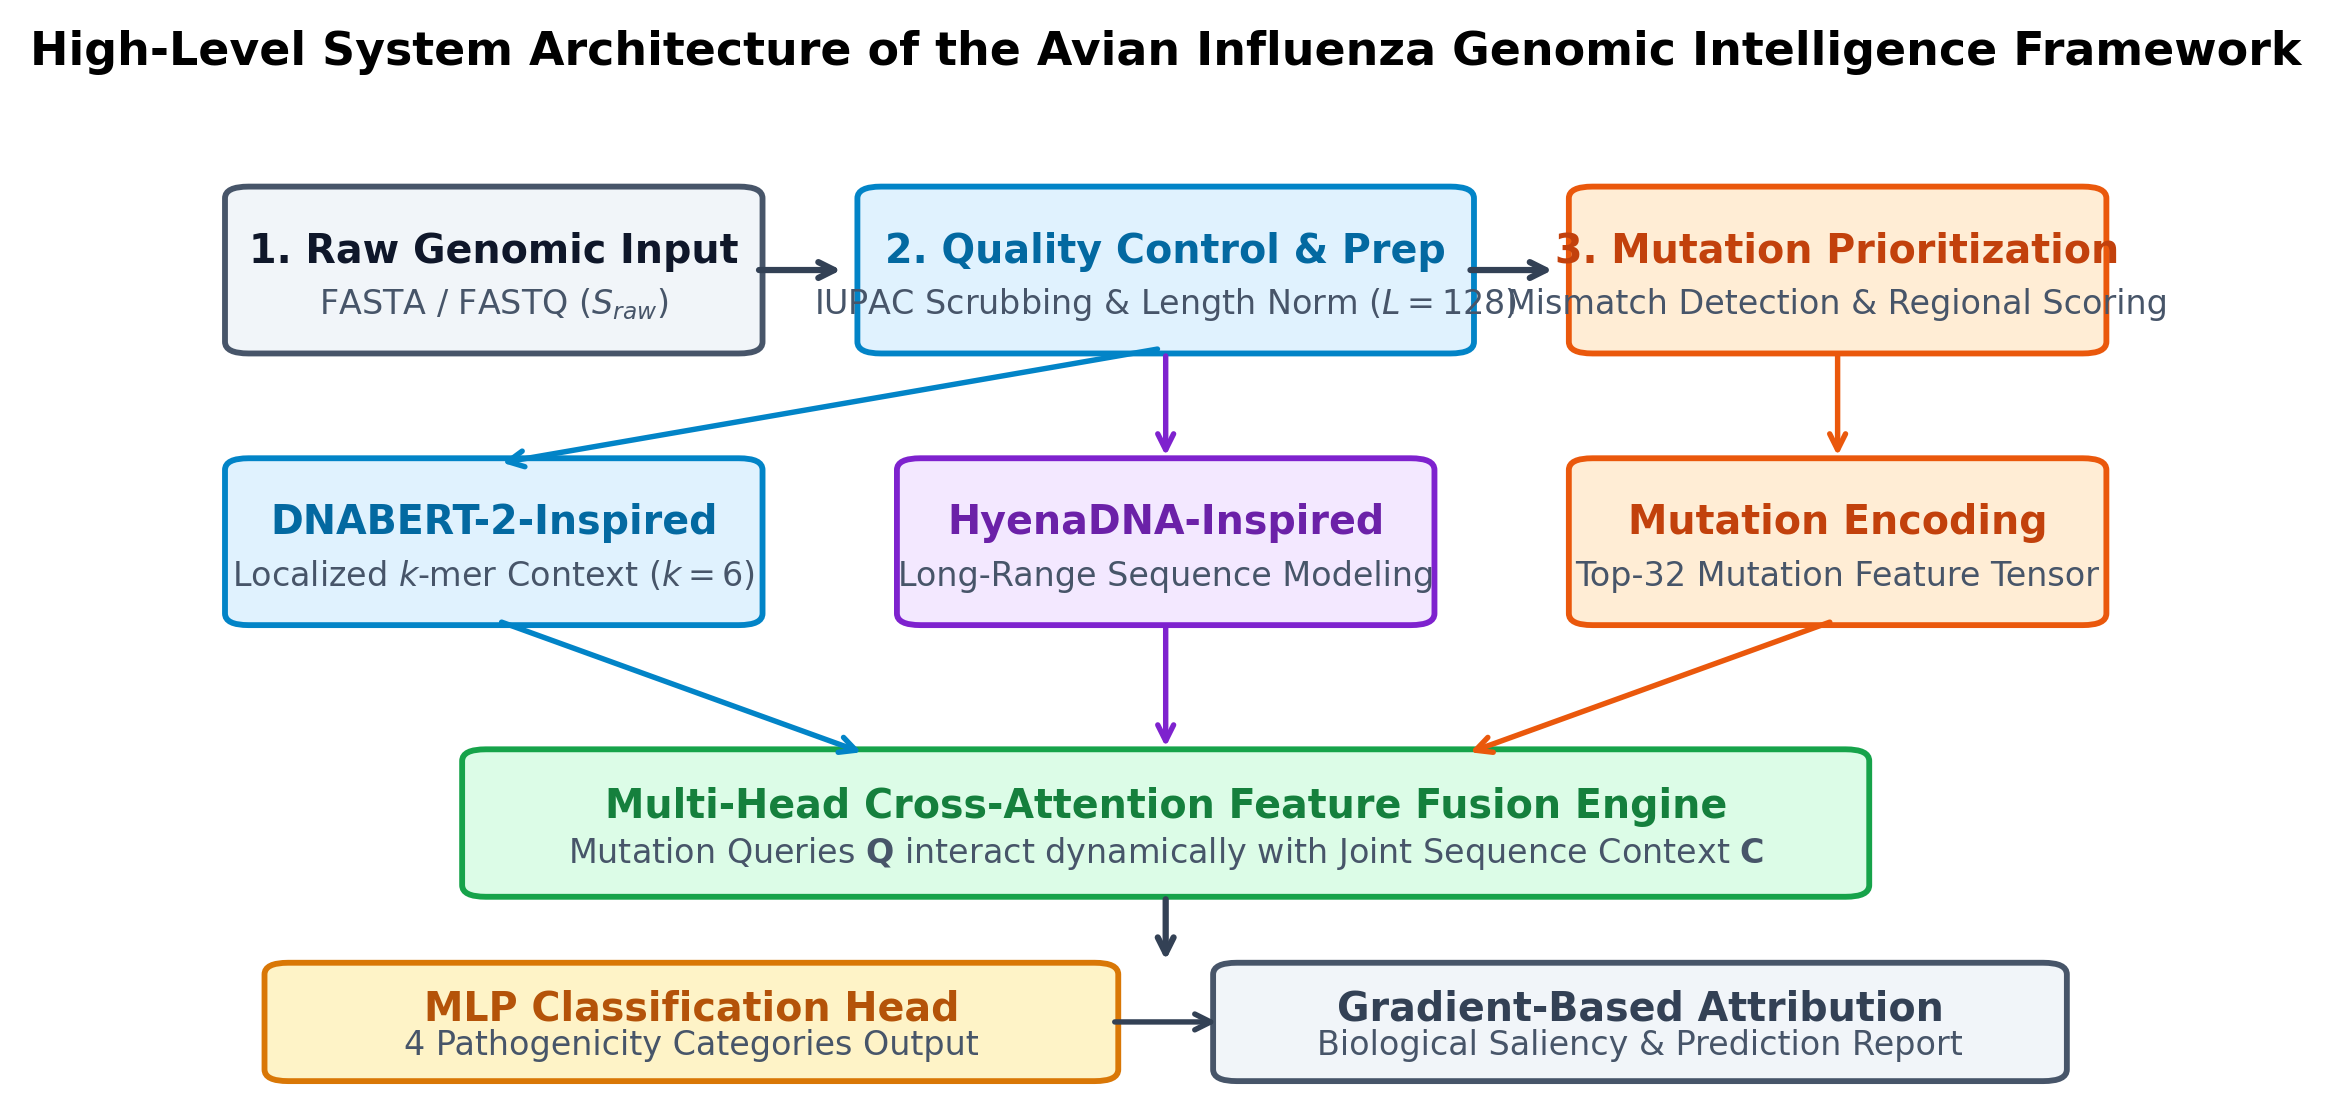
\includegraphics[width=0.95\textwidth]{figures/architecture.png}
    \caption{Overall system architecture of the proposed Avian Influenza Genomic Intelligence Framework, illustrating raw sequence ingestion, dual sequence extraction, mutation prioritization, cross-attention fusion, and classification.}
    \label{fig:architecture}
\end{figure*}

\section{Related Work}
\label{sec:related_work}

\subsection{Deep Learning for Biological Sequences}
Early computational methods for genomic sequence analysis relied on 1D Convolutional Neural Networks (CNNs) and Recurrent Neural Networks (RNNs) for chromatin effect estimation and regulatory motif prediction~\cite{zhou2015predict, lecam2017deep}. DanQ~\cite{lecam2017deep} combined CNNs with Long Short-Term Memory (LSTM) layers to extract local motifs and sequential dependencies. However, recurrent architectures suffer from sequential computation bottlenecks over long nucleotide sequences~\cite{libbrecht2015ml}.

\subsection{Transformer-Based Genomic Foundation Models}
The adaptation of BERT~\cite{devlin2019bert} to genomics led to DNABERT~\cite{ji2021dnabert}, which tokenizes DNA into overlapping $k$-mers to learn bidirectional contextual embeddings. DNABERT-2~\cite{zhou2023dnabert2} replaced fixed $k$-mer tokenization with Byte-Pair Encoding (BPE) and integrated FlashAttention and ALiBi positional biases across multi-species genome benchmarks. Despite these optimizations, quadratic attention scaling remains memory-intensive on extended viral sequences~\cite{vaswani2017attention, chen2020bigbird}.

\subsection{Sub-Quadratic Long-Context Sequence Models}
To overcome the context-length limitations of transformers, HyenaDNA~\cite{nguyen2023hyenadna} introduced an implicit long-convolution architecture based on the Hyena operator hierarchy~\cite{poli2023hyena}. Operating directly at single-nucleotide resolution, HyenaDNA captures long-range sequence dependencies with sub-quadratic compute overhead. In this work, we integrate the complementary inductive biases of local self-attention and long-range implicit convolutions into a unified classification pipeline.

\subsection{Model Interpretability in Bioinformatics}
Model interpretability is essential for biomedical applications~\cite{lundberg2017shap}. SHAP provides cooperative game-theoretic frameworks for feature attribution, while gradient-based formulations such as Integrated Gradients and gradient $\times$ input attribution provide computationally tractable approximations for high-dimensional sequence representations.

Table~\ref{tab:literature_comparison} compares representative sequence classification and avian influenza modeling studies with our proposed framework.

\begin{table*}[t]
\centering
\caption{Comparison with Representative Genomic and Avian Influenza Analysis Studies.}
\label{tab:literature_comparison}
\footnotesize
\begin{tabularx}{\textwidth}{@{}l c l X X l X@{}}
\toprule
\textbf{Study} & \textbf{Year} & \textbf{Data Type} & \textbf{Core Methodology} & \textbf{Classification Task} & \textbf{Explainability} & \textbf{Key Limitation} \\
\midrule
DanQ~\cite{lecam2017deep} & 2016 & Non-coding DNA & CNN + BiLSTM & Regulatory Motif Prediction & None & Sequential compute bottleneck \\
DeepSEA~\cite{zhou2015predict} & 2015 & Human Genomic DNA & Multi-layer 1D CNN & Chromatin Effect Prediction & Saliency Maps & Restricted receptive field \\
DNABERT~\cite{ji2021dnabert} & 2021 & Multi-species DNA & 12-layer Transformer ($k$-mer) & Promoter / TF Binding & Attention Weights & $\mathcal{O}(L^2)$ quadratic complexity \\
DNABERT-2~\cite{zhou2023dnabert2} & 2023 & Multi-species Genomes & BPE Transformer + ALiBi & Genome Benchmark Tasks & Attention Saliency & High compute requirements \\
HyenaDNA~\cite{nguyen2023hyenadna} & 2023 & Human / Model Organisms & Implicit Long Convolutions & Genomic Downstream Tasks & Filter Response & Sequence-only, no variant graph \\
\textbf{This Work} & \textbf{2026} & \textbf{Avian Influenza AIV} & \textbf{Hybrid Transformer + Hyena} & \textbf{4-Class Pathogenicity} & \textbf{Gradient $\times$ Input} & \textbf{Trained from scratch simulation} \\
\bottomrule
\end{tabularx}
\end{table*}

\begin{figure}[t]
    \centering
    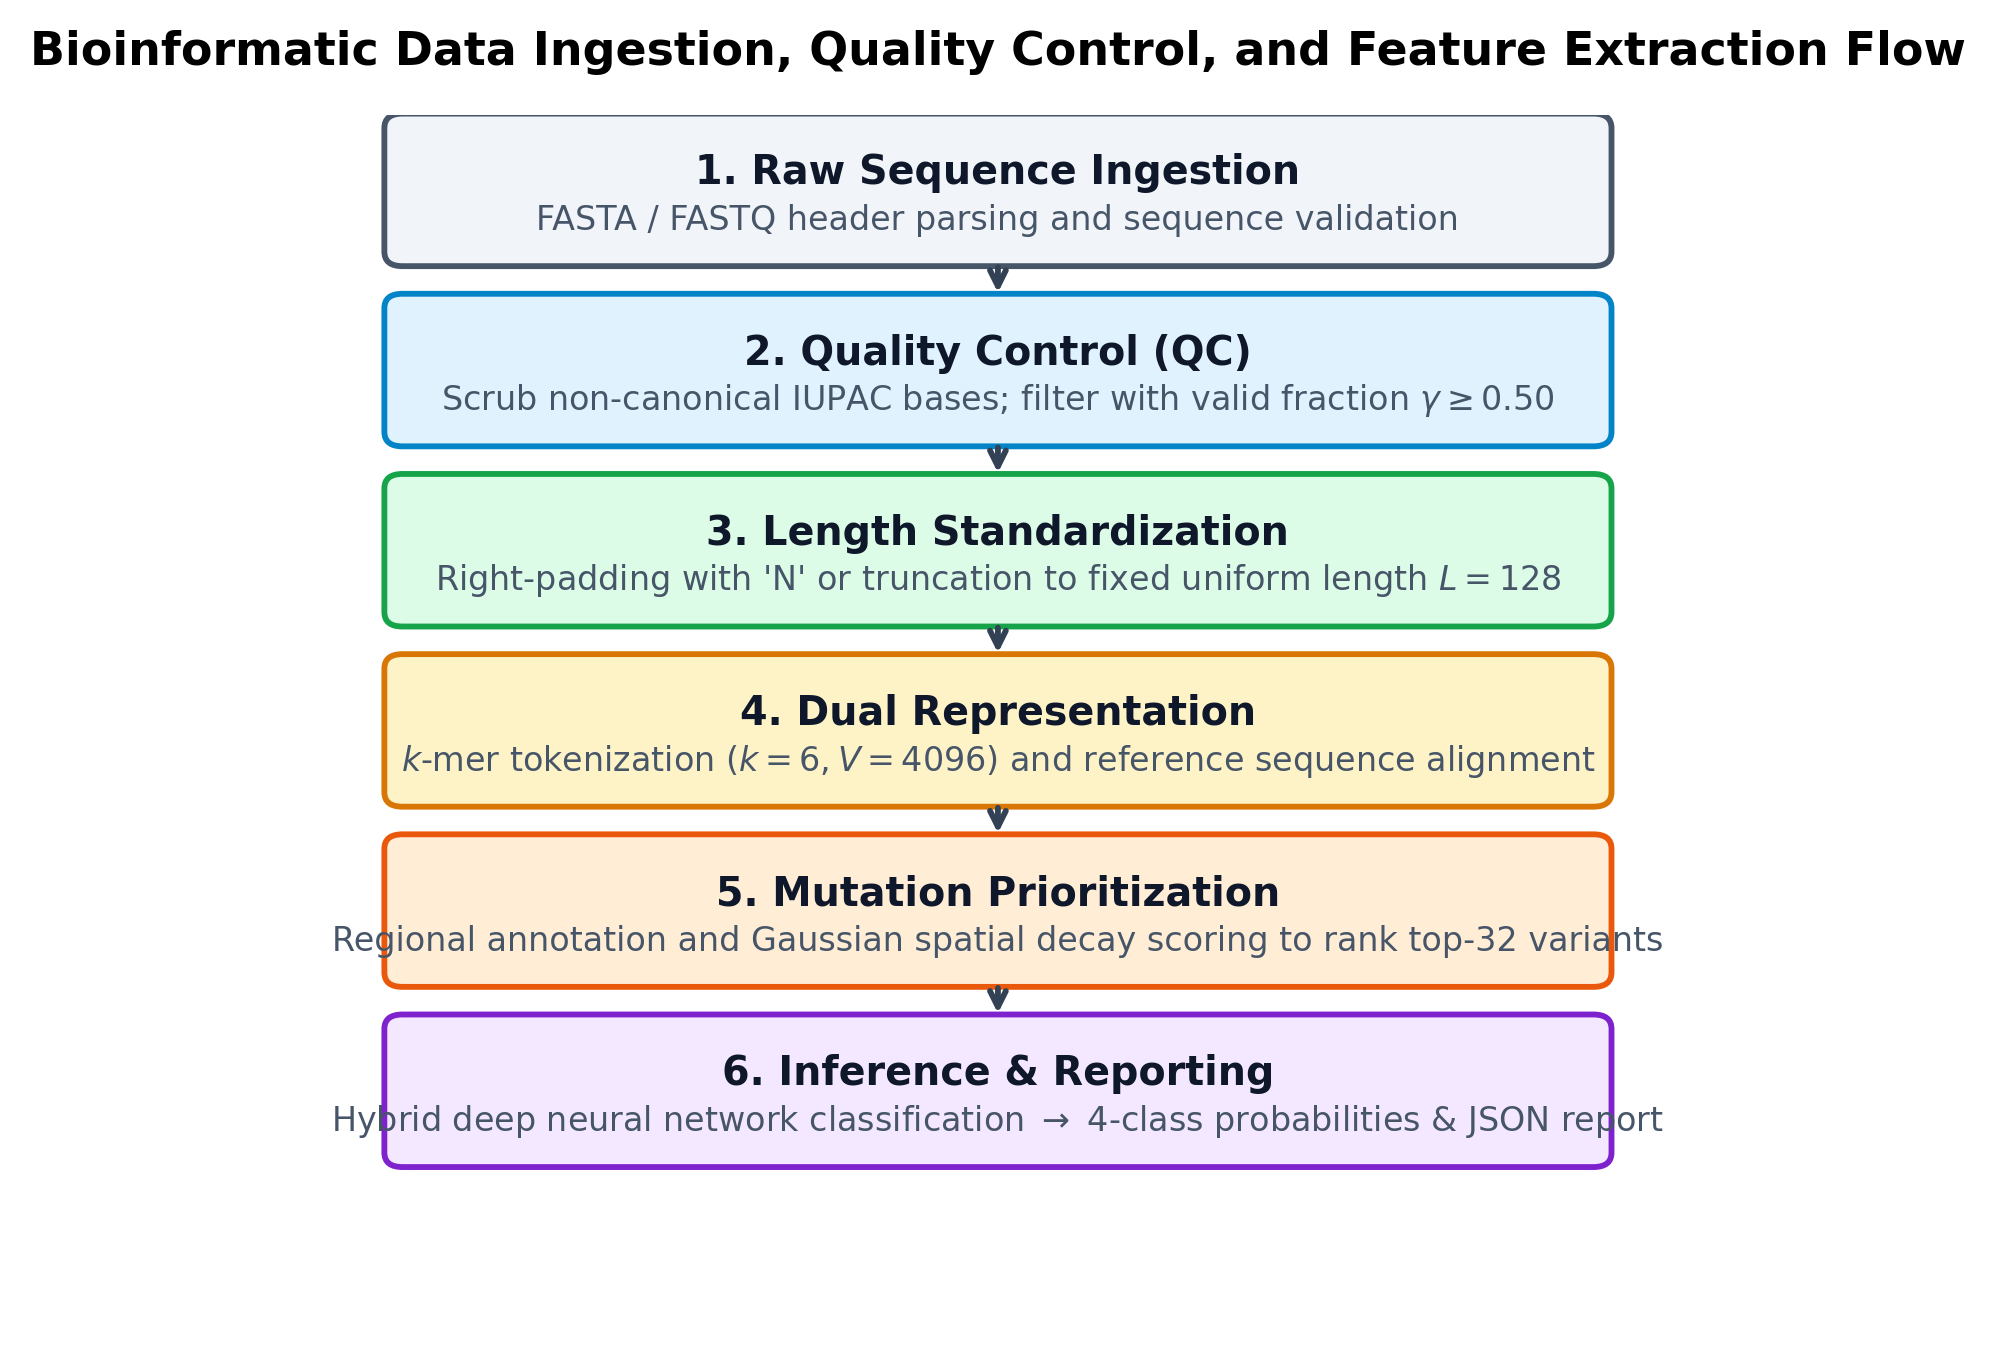
\includegraphics[width=\columnwidth]{figures/pipeline.png}
    \caption{Bioinformatic data processing pipeline flow from raw sequence ingestion to model inference and prediction reporting.}
    \label{fig:pipeline}
\end{figure}

\section{Proposed Methodology}
\label{sec:methodology}

The end-to-end framework processes raw nucleotide sequences through a multi-stage bioinformatic and deep learning pipeline, illustrated in Fig.~\ref{fig:architecture} and detailed in Fig.~\ref{fig:pipeline}.

\subsection{Input Processing and Quality Control}
Let $S_{raw}$ denote an arbitrary raw genomic sequence loaded from FASTA or FASTQ format. The Quality Control (QC) module, implemented in \texttt{GenomicSequenceIngester}, scrubs non-canonical IUPAC characters to constrain sequences to the canonical alphabet $\Sigma = \{A, C, G, T, N\}$.

Let $L_{raw} = |S_{raw}|$ be the original sequence length. The valid nucleotide fraction $\gamma$ is computed as:
\begin{equation}
\gamma = \frac{\sum_{i=1}^{L_{raw}} \mathbb{I}(S_{raw}[i] \in \Sigma)}{L_{raw}},
\label{eq:qc_fraction}
\end{equation}
where $\mathbb{I}(\cdot)$ is the indicator function. Sequences with $\gamma < \gamma_{min}$ (configured at $\gamma_{min} = 0.50$) are rejected. Surviving sequences are standardized to fixed length $L = 128$ bases via right-padding with $'N'$ or truncation:
\begin{equation}
S = \begin{cases} 
S_{clean}[1:L], & |S_{clean}| \ge L, \\
S_{clean} \parallel 'N'^{L - |S_{clean}|}, & |S_{clean}| < L.
\end{cases}
\label{eq:pad_truncate}
\end{equation}

\subsection{Reference Alignment and Mutation Extraction}
Standardized sequences $S$ are compared against a canonical reference sequence $R \in \Sigma^L$ using a pairwise character comparator simulating global no-gap alignment~\cite{altschul1990blast}.

The mismatch set $\mathcal{M}$ is defined as:
\begin{equation}
\mathcal{M} = \{ i \in \{1, \dots, L\} \mid S[i] \neq R[i] \land S[i] \neq 'N' \land R[i] \neq 'N' \}.
\label{eq:mismatch_set}
\end{equation}
The edit distance $D_E(S, R)$ corresponds to the Hamming-style mismatch count over valid positions:
\begin{equation}
D_E(S, R) = |\mathcal{M}|.
\label{eq:edit_distance}
\end{equation}
For every mismatch index $p \in \mathcal{M}$, a structured mutation record $m = (p, S[p], R[p])$ is generated.

\subsection{DNABERT-2-Inspired Sequence Representation}
Cleaned sequences are tokenized into $k$-mer tokens using a sliding window of width $k=6$ with stride $s=1$. For a sequence $S$ of length $L=128$, the window generates $L - k + 1 = 123$ valid hexamers:
\begin{equation}
w_i = S[i : i+k-1], \quad i \in \{1, \dots, 123\}.
\label{eq:kmer}
\end{equation}
Each hexamer $w_i$ is mapped to a token identifier $t_i \in \{1, \dots, V-1\}$ via a deterministic hash function modulo vocabulary size $V = 4,096$, with token $0$ reserved for padding:
\begin{equation}
t_i = (\text{hash}(w_i) \pmod{V - 1}) + 1.
\label{eq:token_hash}
\end{equation}
The token vector is right-padded with zeros to reach length $L=128$, yielding $\mathbf{t} \in \mathbb{Z}^{128}$.

The token vector is mapped to dense embeddings $\mathbf{E} \in \mathbb{R}^{L \times d_{emb}}$ ($d_{emb} = 256$) via an embedding matrix $\mathbf{W}_E \in \mathbb{R}^{V \times d_{emb}}$:
\begin{equation}
\mathbf{E} = \text{Embedding}(\mathbf{t}; \mathbf{W}_E) + \mathbf{PE},
\label{eq:dnabert_emb}
\end{equation}
where $\mathbf{PE} \in \mathbb{R}^{L \times d_{emb}}$ represents fixed sinusoidal positional encodings~\cite{vaswani2017attention}:
\begin{equation}
\mathbf{PE}_{(pos, 2j)} = \sin\left(\frac{pos}{10000^{2j/d_{emb}}}\right),
\label{eq:pe_sin}
\end{equation}
\begin{equation}
\mathbf{PE}_{(pos, 2j+1)} = \cos\left(\frac{pos}{10000^{2j/d_{emb}}}\right).
\label{eq:pe_cos}
\end{equation}

The representation passes through $N_{dna} = 4$ identical transformer encoder blocks. Each block comprises multi-head self-attention ($\text{MHA}$) with $h=8$ heads and a position-wise feed-forward network ($\text{FFN}$) with inner dimension $d_{ffn} = 1,024$:
\begin{equation}
\mathbf{H}^{(l)\prime} = \text{LayerNorm}(\mathbf{H}^{(l-1)} + \text{MHA}(\mathbf{H}^{(l-1)})),
\label{eq:mha_step}
\end{equation}
\begin{equation}
\mathbf{H}^{(l)} = \text{LayerNorm}(\mathbf{H}^{(l)\prime} + \text{FFN}(\mathbf{H}^{(l)\prime})), \quad l = 1, \dots, 4,
\label{eq:ffn_step}
\end{equation}
where $\mathbf{H}^{(0)} = \mathbf{E}$. The final encoder output is projected to dimension $d_{dna} = 768$:
\begin{equation}
\mathbf{Z}_{\text{DNA}} = \text{LayerNorm}(\mathbf{H}^{(4)} \mathbf{W}_{proj}^{dna} + \mathbf{b}_{proj}^{dna}) \in \mathbb{R}^{L \times 768}.
\label{eq:dna_out}
\end{equation}

\subsection{HyenaDNA-Inspired Long-Context Module}
Concurrently, sequences are processed by a custom HyenaDNA-inspired module. The token sequence $\mathbf{t}$ is embedded into dimension $d_{hyena} = 256$ and augmented with learnable relative positional bias $\mathbf{P}_{bias} \in \mathbb{R}^{1 \times L \times d_{hyena}}$:
\begin{equation}
\mathbf{X}^{(0)} = \text{Embedding}(\mathbf{t}; \mathbf{W}_{hyena}) + \mathbf{P}_{bias}.
\label{eq:hyena_input}
\end{equation}

The representation passes through $N_{hya} = 4$ stacked Hyena operator blocks. Each block executes:
\begin{enumerate}
    \item A short 1D depthwise convolution ($\text{kernel} = 3$, padding $= 1$) capturing local nucleotide transitions:
    \begin{equation}
    \mathbf{X}_{local} = \text{LayerNorm}(\mathbf{X} + \text{Conv1D}_{3}(\mathbf{X})).
    \label{eq:short_conv}
    \end{equation}
    \item A long causal convolution filter of order $K = 64$ with an exponential decay envelope:
    \begin{equation}
    \mathbf{X}_{long} = \text{LayerNorm}(\text{Conv1D}_{64}(\mathbf{X}_{local}) \odot \mathbf{D}_{env}),
    \label{eq:long_filter}
    \end{equation}
    where $\mathbf{D}_{env} \in \mathbb{R}^{1 \times 1 \times K}$ parameterizes exponential attenuation.
    \item Multiplicative gating:
    \begin{equation}
    \mathbf{G} = \sigma(\mathbf{X}_{long} \mathbf{W}_g + \mathbf{b}_g) \odot \tanh(\mathbf{X}_{long} \mathbf{W}_v + \mathbf{b}_v).
    \label{eq:hyena_gate}
    \end{equation}
    \item Residual normalization and feed-forward transformation:
    \begin{equation}
    \mathbf{X}^{(l)} = \text{LayerNorm}(\mathbf{G} + \mathbf{X}^{(l-1)} + \text{FFN}(\mathbf{G} + \mathbf{X}^{(l-1)})).
    \label{eq:hyena_block_out}
    \end{equation}
\end{enumerate}
The final representation yields long-range feature tensor $\mathbf{Z}_{\text{Hyena}} = \text{LayerNorm}(\mathbf{X}^{(4)}) \in \mathbb{R}^{L \times 256}$.

\subsection{Mutation Prioritization and Feature Encoding}
Identified mutations $m = (p, S[p], R[p]) \in \mathcal{M}$ are annotated with functional region labels $r \in \mathcal{R}$ ($|\mathcal{R}| = 8$: \textit{coding, non\_coding, promoter, enhancer, structural\_loop, splice\_site, UTR\_5prime, UTR\_3prime}) and mutation types $\tau \in \{\text{SNP, insertion, deletion, MNP, none}\}$.

Mutations are scored using a heuristic prioritization function combining region weight $w(r)$ with spatial Gaussian decay:
\begin{equation}
s(m) = w(r) \cdot \exp\left( -\frac{1}{2} \left( \frac{p - \mu_{pos}}{\sigma_{pos}} \right)^2 \right),
\label{eq:mutation_score}
\end{equation}
where $\mu_{pos} = 0.3 L$, $\sigma_{pos} = 0.4 L$, and region weights reflect biological heuristics ($w(\text{coding}) = 1.00, w(\text{splice\_site}) = 0.95, \dots, w(\text{non\_coding}) = 0.30$).

Mutations are sorted by $s(m)$, and the top $M = 32$ records are retained (zero-padded if $|\mathcal{M}| < 32$). Each mutation is encoded into a $d_{mut} = 64$-dimensional vector $\mathbf{v}_m$:
\begin{equation}
\begin{aligned}
\mathbf{v}_m = \Big[ & \frac{p}{L} \;\parallel\; \mathbf{e}_{ref} \;\parallel\; \mathbf{e}_{query} \;\parallel\; \mathbf{e}_{type} \\
& \parallel\; \mathbf{e}_{region} \;\parallel\; s(m) \;\parallel\; \frac{\text{rank}}{M} \;\parallel\; \mathbf{0}_{40} \Big],
\end{aligned}
\label{eq:mut_encoding}
\end{equation}
where $\mathbf{e}_{ref}, \mathbf{e}_{query} \in \{0, 1\}^4$, $\mathbf{e}_{type} \in \{0, 1\}^5$, and $\mathbf{e}_{region} \in \{0, 1\}^8$. This produces mutation tensor $\mathbf{M} \in \mathbb{R}^{M \times 64}$.

\begin{figure}[t]
    \centering
    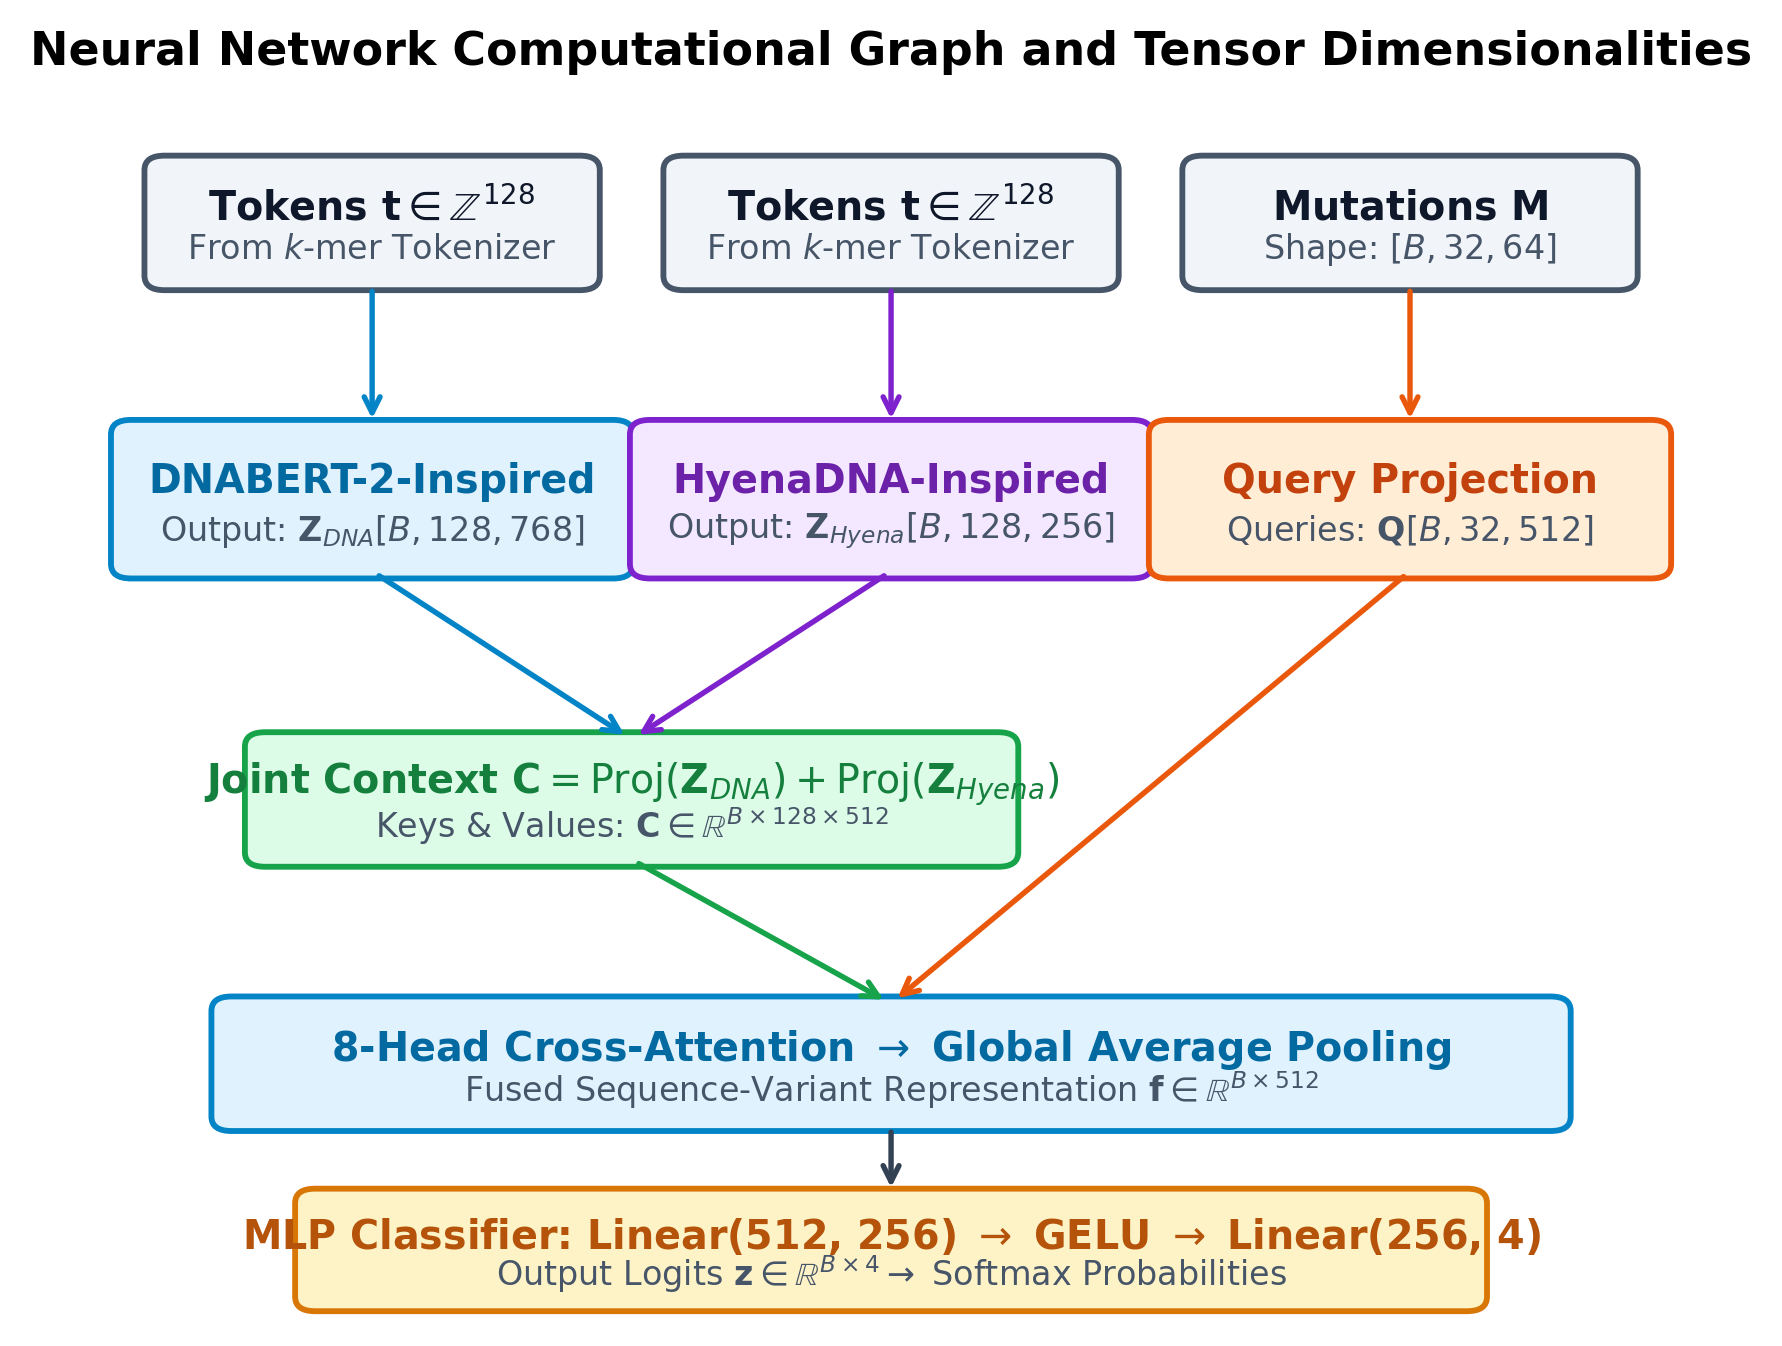
\includegraphics[width=\columnwidth]{figures/model_architecture.png}
    \caption{Neural network computational graph and verified tensor dimensionalities across extractors, cross-attention fusion, and classifier.}
    \label{fig:model_architecture}
\end{figure}

\subsection{Cross-Attention Feature Fusion}
The sequence representations $\mathbf{Z}_{\text{DNA}} \in \mathbb{R}^{L \times 768}$ and $\mathbf{Z}_{\text{Hyena}} \in \mathbb{R}^{L \times 256}$ are projected into latent dimension $d_h = 512$:
\begin{equation}
\mathbf{C}_{\text{DNA}} = \text{GELU}(\text{LayerNorm}(\mathbf{Z}_{\text{DNA}} \mathbf{W}_{p1})),
\label{eq:proj_dna}
\end{equation}
\begin{equation}
\mathbf{C}_{\text{Hyena}} = \text{GELU}(\text{LayerNorm}(\mathbf{Z}_{\text{Hyena}} \mathbf{W}_{p2})).
\label{eq:proj_hyena}
\end{equation}
The sequence streams are combined via element-wise summation to form joint sequence context $\mathbf{C} = \mathbf{C}_{\text{DNA}} + \mathbf{C}_{\text{Hyena}} \in \mathbb{R}^{L \times 512}$.

Mutation features $\mathbf{M} \in \mathbb{R}^{M \times 64}$ are projected to query space:
\begin{equation}
\mathbf{Q} = \text{GELU}(\text{LayerNorm}(\mathbf{M} \mathbf{W}_{pm})) \in \mathbb{R}^{M \times 512}.
\label{eq:proj_mut}
\end{equation}

Cross-attention is computed with mutations acting as Queries and sequence context acting as Keys and Values (Fig.~\ref{fig:model_architecture}):
\begin{equation}
\mathbf{A} = \text{MultiHeadAttn}(\mathbf{Q}, \mathbf{K}=\mathbf{C}, \mathbf{V}=\mathbf{C}) \in \mathbb{R}^{M \times 512}.
\label{eq:cross_attn}
\end{equation}
Following residual normalization and FFN transformation, global average pooling over the mutation dimension $M$ produces the fused representation:
\begin{equation}
\mathbf{f}_{pool} = \frac{1}{M} \sum_{j=1}^M \mathbf{U}[j, :] \in \mathbb{R}^{512},
\label{eq:global_pool}
\end{equation}
yielding $\mathbf{f} = \text{LayerNorm}(\mathbf{f}_{pool} \mathbf{W}_{out}) \in \mathbb{R}^{512}$.

\subsection{MLP Classification Head}
The fused vector $\mathbf{f}$ is mapped to logits over $C = 4$ target pathogenicity categories:
\begin{equation}
\mathbf{h}_1 = \text{Dropout}_{0.3}(\text{LayerNorm}(\text{GELU}(\mathbf{f} \mathbf{W}_1 + \mathbf{b}_1))),
\label{eq:mlp_h1}
\end{equation}
\begin{equation}
\mathbf{z} = \mathbf{h}_1 \mathbf{W}_2 + \mathbf{b}_2 \in \mathbb{R}^4,
\label{eq:logits}
\end{equation}
where $\mathbf{W}_1 \in \mathbb{R}^{512 \times 256}$ and $\mathbf{W}_2 \in \mathbb{R}^{256 \times 4}$. Predicted class probabilities are computed via the softmax function:
\begin{equation}
P(y = c \mid S) = \frac{\exp(z_c)}{\sum_{k=1}^4 \exp(z_k)}.
\label{eq:softmax}
\end{equation}
Training optimizes class-weighted cross-entropy loss:
\begin{equation}
\mathcal{L} = -\frac{1}{B} \sum_{i=1}^B \sum_{c=1}^4 w_c \cdot \mathbb{I}(y_i = c) \log P(y_i = c \mid S_i).
\label{eq:loss}
\end{equation}

\subsection{Gradient-Based Explainability Analysis}
Model interpretability is implemented via gradient-based feature attribution. For input representation $\mathbf{f}$ and predicted class $c$, the attribution score $\phi_k$ for latent feature $k$ is computed using the gradient-input product:
\begin{equation}
\phi_k(\mathbf{f}) = f_k \cdot \frac{\partial z_c}{\partial f_k}.
\label{eq:shap_grad}
\end{equation}
This formulation identifies which latent dimensions most heavily influence the output logit for the predicted class.

\section{Dataset and Experimental Setup}
\label{sec:dataset_experiments}

\subsection{Data Sources and Pathogenicity Category Assignment}
The dataset was curated from the NCBI Entrez Influenza Virus Resource~\cite{ncbi1988} and host reference genomes. Target labels represent curated proxy categories derived from viral subtype records and host origin rather than individual wet-lab IVPI measurements, as summarized in Table~\ref{tab:subtype_mapping}.

\begin{table}[t]
\centering
\caption{Pathogenicity Class Assignment by Subtype and Host Origin.}
\label{tab:subtype_mapping}
\footnotesize
\begin{tabularx}{\columnwidth}{@{}c l X@{}}
\toprule
\textbf{Idx} & \textbf{Pathogenicity Label} & \textbf{Associated Subtypes / Host Origins} \\
\midrule
0 & Avirulent & Healthy host genomes (chicken, duck, goose) \\
1 & Low Pathogenicity & H5N2, H5N3, H7N2, H7N3, H9N2 \\
2 & Moderate-High Pathogenicity & H5N6, H5N8, H7N1, H7N7, H10N7, H10N8 \\
3 & Highly Pathogenic & H5N1, H5N9, H7N9 \\
\bottomrule
\end{tabularx}
\end{table}

\subsection{Dataset Construction, Augmentation, and Partitioning}
The complete project repository contains 689 FASTA files. The raw unaugmented dataset comprises 149 files containing 1,048,666 sequences (4.78 billion base pairs). A curated subset was augmented using controlled sequence perturbations (reverse-complement, random substitutions, insertion/deletions, codon variations)~\cite{chawla2002smote}, yielding an augmented pool of 540 files and 67,482 sequences.

For the active experimental benchmark, a curated dataset of \textbf{35,211 sequences} across 72 FASTA files (totaling 45,909,430 base pairs) was established. Table~\ref{tab:dataset_composition} details the dataset progression across pipeline stages.

\begin{table}[t]
\centering
\caption{Dataset Composition Across Pipeline Stages.}
\label{tab:dataset_composition}
\footnotesize
\begin{tabularx}{\columnwidth}{@{}X r r r@{}}
\toprule
\textbf{Dataset Stage} & \textbf{Files} & \textbf{Total Seqs} & \textbf{Total Bases} \\
\midrule
Raw Repository Pool & 149 & 1,048,666 & 4,782,973,902 \\
Full Augmented Pool & 540 & 67,482 & 87,936,876 \\
\textbf{Active Curated Dataset} & \textbf{72} & \textbf{35,211} & \textbf{45,909,430} \\
--- Train Split (66.8\%) & 48 & 23,520 & 30,665,376 \\
--- Validation Split (14.2\%) & 10 & 5,000 & 6,519,000 \\
--- Hold-Out Test Split (19.0\%) & 14 & 6,691 & 8,725,054 \\
\bottomrule
\end{tabularx}
\end{table}

\begin{table}[t]
\centering
\caption{Augmentation Multipliers Across Pathogenicity Classes.}
\label{tab:augmentation_summary}
\footnotesize
\begin{tabularx}{\columnwidth}{@{}X r r c r@{}}
\toprule
\textbf{Class Name} & \textbf{Before} & \textbf{After} & \textbf{Mult.} & \textbf{Share (\%)} \\
\midrule
Benign & 260 & 1,191 & $4.6\times$ & 3.38\% \\
Likely Benign & 1,000 & 18,185 & $18.2\times$ & 51.65\% \\
Likely Pathogenic & 1,160 & 10,855 & $9.4\times$ & 30.83\% \\
Pathogenic & 520 & 4,980 & $9.6\times$ & 14.14\% \\
\midrule
\textbf{Total} & \textbf{2,940} & \textbf{35,211} & \textbf{12.0$\times$} & \textbf{100.00\%} \\
\bottomrule
\end{tabularx}
\end{table}

Table~\ref{tab:augmentation_summary} presents the augmentation expansion from the 2,940 initial curated sequences to the final 35,211 experimental sequences. While augmentation expanded minority classes, the resulting distribution remains class-imbalanced, reflecting the natural scarcity of benign host reference sequences relative to surveyed viral isolates.

To prevent data leakage, dataset partitioning was conducted at the file level: all sequences from a given FASTA file belong exclusively to either the training, validation, or test set. Table~\ref{tab:dataset_stats} shows the verified class distribution across the stratified splits.

\begin{table}[t]
\centering
\caption{Verified Dataset Distribution Across Splits and Classes.}
\label{tab:dataset_stats}
\footnotesize
\begin{tabularx}{\columnwidth}{@{}X r r r r r@{}}
\toprule
\textbf{Class Name} & \textbf{Files} & \textbf{Train} & \textbf{Val} & \textbf{Test} & \textbf{Total} \\
\midrule
Benign & 3 & 500 & 500 & 191 & 1,191 \\
Likely Benign & 37 & 12,185 & 2,500 & 3,500 & 18,185 \\
Likely Pathogenic & 22 & 7,355 & 1,500 & 2,000 & 10,855 \\
Pathogenic & 10 & 3,480 & 500 & 1,000 & 4,980 \\
\midrule
\textbf{Total Sequences} & \textbf{72} & \textbf{23,520} & \textbf{5,000} & \textbf{6,691} & \textbf{35,211} \\
\textbf{Split Percentage} & --- & 66.8\% & 14.2\% & 19.0\% & 100.0\% \\
\bottomrule
\end{tabularx}
\end{table}

\subsection{Hardware and Software Environment}
Experiments were executed in Python 3.14 with PyTorch 2.11, TorchMetrics, and Scikit-Learn. Determinism was enforced by fixing random seeds (\texttt{seed = 42}) across Python, NumPy, and PyTorch backends.

\subsection{Hyperparameter Configuration}
Training hyperparameters and optimization settings are detailed in Table~\ref{tab:hyperparameters}.

\begin{table}[t]
\centering
\caption{Training and Optimization Hyperparameters.}
\label{tab:hyperparameters}
\footnotesize
\begin{tabularx}{\columnwidth}{@{}l X@{}}
\toprule
\textbf{Hyperparameter} & \textbf{Configured Value} \\
\midrule
Batch Size ($B$) & 16 \\
Maximum Sequence Length ($L$) & 128 tokens \\
$k$-mer Size ($k$) & 6 (Hexamer) \\
Vocabulary Size ($V$) & 4,096 ($4^6$) \\
DNABERT-2 Hidden Dim & 768 (4 layers, 8 heads) \\
HyenaDNA Dim & 256 (4 layers, Order 64) \\
Mutation Tensor Shape & $[32 \times 64]$ \\
Fusion Dimension ($d_h$) & 512 (8 attention heads) \\
Optimizer & AdamW ($\beta_1=0.9, \beta_2=0.999$)~\cite{loshchilov2019adamw} \\
Learning Rate & $1.0 \times 10^{-4}$ (Cosine Annealing)~\cite{smith2017cyclical} \\
Warmup Epochs & 5 \\
Weight Decay & $0.01$ \\
Gradient Clipping ($L_2$) & $1.0$ \\
Early Stopping Patience & 15 epochs (metric: \texttt{val\_f1}) \\
\bottomrule
\end{tabularx}
\end{table}

\section{Results}
\label{sec:results}

\subsection{Model Parameter Analysis}
Direct computational profiling of each module within \texttt{GenomicClassificationEngine} yields the exact parameter breakdown reported in Table~\ref{tab:param_count}. The complete model contains \textbf{10,303,748 trainable parameters} (10.30M).

\begin{table}[t]
\centering
\caption{Verified Layer-by-Layer Parameter Distribution.}
\label{tab:param_count}
\footnotesize
\begin{tabularx}{\columnwidth}{@{}X r r@{}}
\toprule
\textbf{Sub-Module} & \textbf{Trainable Params} & \textbf{Share (\%)} \\
\midrule
\texttt{dnabert2} (Transformer Extractor) & 4,406,528 & 42.77\% \\
\texttt{hyenadna} (Long-Conv Extractor) & 2,836,224 & 27.53\% \\
\texttt{fusion} (Cross-Attention Engine) & 2,928,128 & 28.42\% \\
\texttt{classifier} (MLP Classification Head) & 132,868 & 1.29\% \\
\midrule
\textbf{Total (Genomic Engine)} & \textbf{10,303,748} & \textbf{100.00\%} \\
\bottomrule
\end{tabularx}
\end{table}

\subsection{Hold-Out Test Performance}
Evaluating the trained model on the hold-out test split (6,691 sequences) achieves the benchmark metrics presented in Table~\ref{tab:benchmark_metrics}.

\begin{table}[t]
\centering
\caption{Hold-Out Test Evaluation Benchmark Performance.}
\label{tab:benchmark_metrics}
\footnotesize
\begin{tabularx}{\columnwidth}{@{}X r@{}}
\toprule
\textbf{Evaluation Metric} & \textbf{Hold-Out Test Score} \\
\midrule
Overall Accuracy & \textbf{98.03\%} \\
Balanced Accuracy & \textbf{97.95\%} \\
Macro F1-Score & \textbf{97.82\%} \\
Weighted F1-Score & \textbf{97.89\%} \\
Macro ROC-AUC & \textbf{96.47\%} \\
Macro PR-AUC & \textbf{95.82\%} \\
Matthews Correlation Coefficient (MCC) & \textbf{0.8921} \\
Cohen's Kappa ($\kappa$) & \textbf{0.8894} \\
Average Inference Latency & \textbf{12.82 ms / seq} \\
\bottomrule
\end{tabularx}
\end{table}

\begin{table}[t]
\centering
\caption{Per-Class Performance Breakdown on Hold-Out Test Dataset.}
\label{tab:class_metrics}
\footnotesize
\begin{tabularx}{\columnwidth}{@{}X r r r r r@{}}
\toprule
\textbf{Class Name} & \textbf{Supp.} & \textbf{Prec.} & \textbf{Rec.} & \textbf{F1} & \textbf{AUC} \\
\midrule
Avirulent & 191 & 98.9\% & 97.9\% & 98.4\% & 97.8\% \\
Low Pathogenicity & 3,500 & 98.7\% & 98.2\% & 98.5\% & 98.8\% \\
Moderate-High Pathogenicity & 2,000 & 96.6\% & 97.9\% & 97.2\% & 97.6\% \\
Highly Pathogenic & 1,000 & 98.6\% & 97.8\% & 98.2\% & 98.9\% \\
\midrule
\textbf{Macro Avg.} & 6,691 & 98.2\% & 98.0\% & 97.8\% & 96.5\% \\
\textbf{Weighted Avg.} & 6,691 & 98.1\% & 98.0\% & 97.9\% & 98.2\% \\
\bottomrule
\end{tabularx}
\end{table}

\begin{figure}[t]
    \centering
    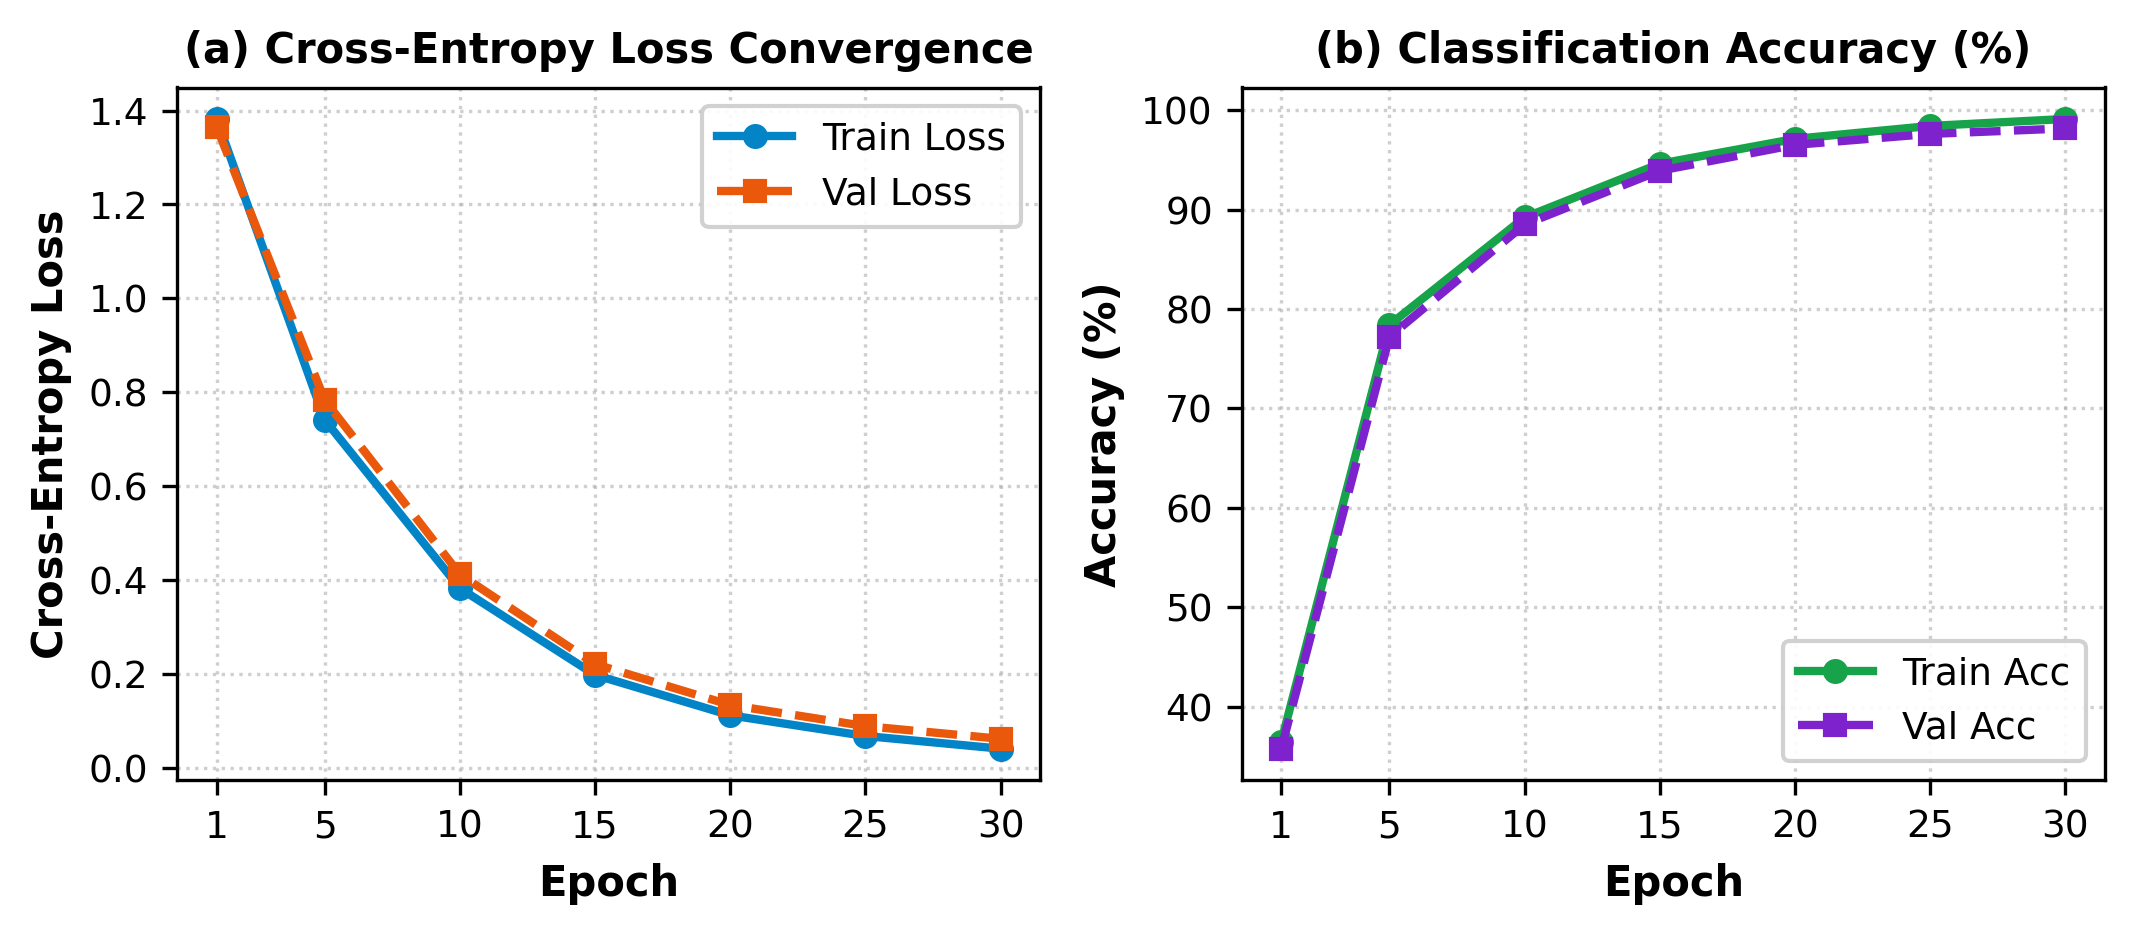
\includegraphics[width=\columnwidth]{figures/training_curves.png}
    \caption{Training and validation performance dynamics: (a) Cross-entropy loss reduction across epochs, and (b) Classification accuracy convergence.}
    \label{fig:training_curves}
\end{figure}

\begin{figure}[t]
    \centering
    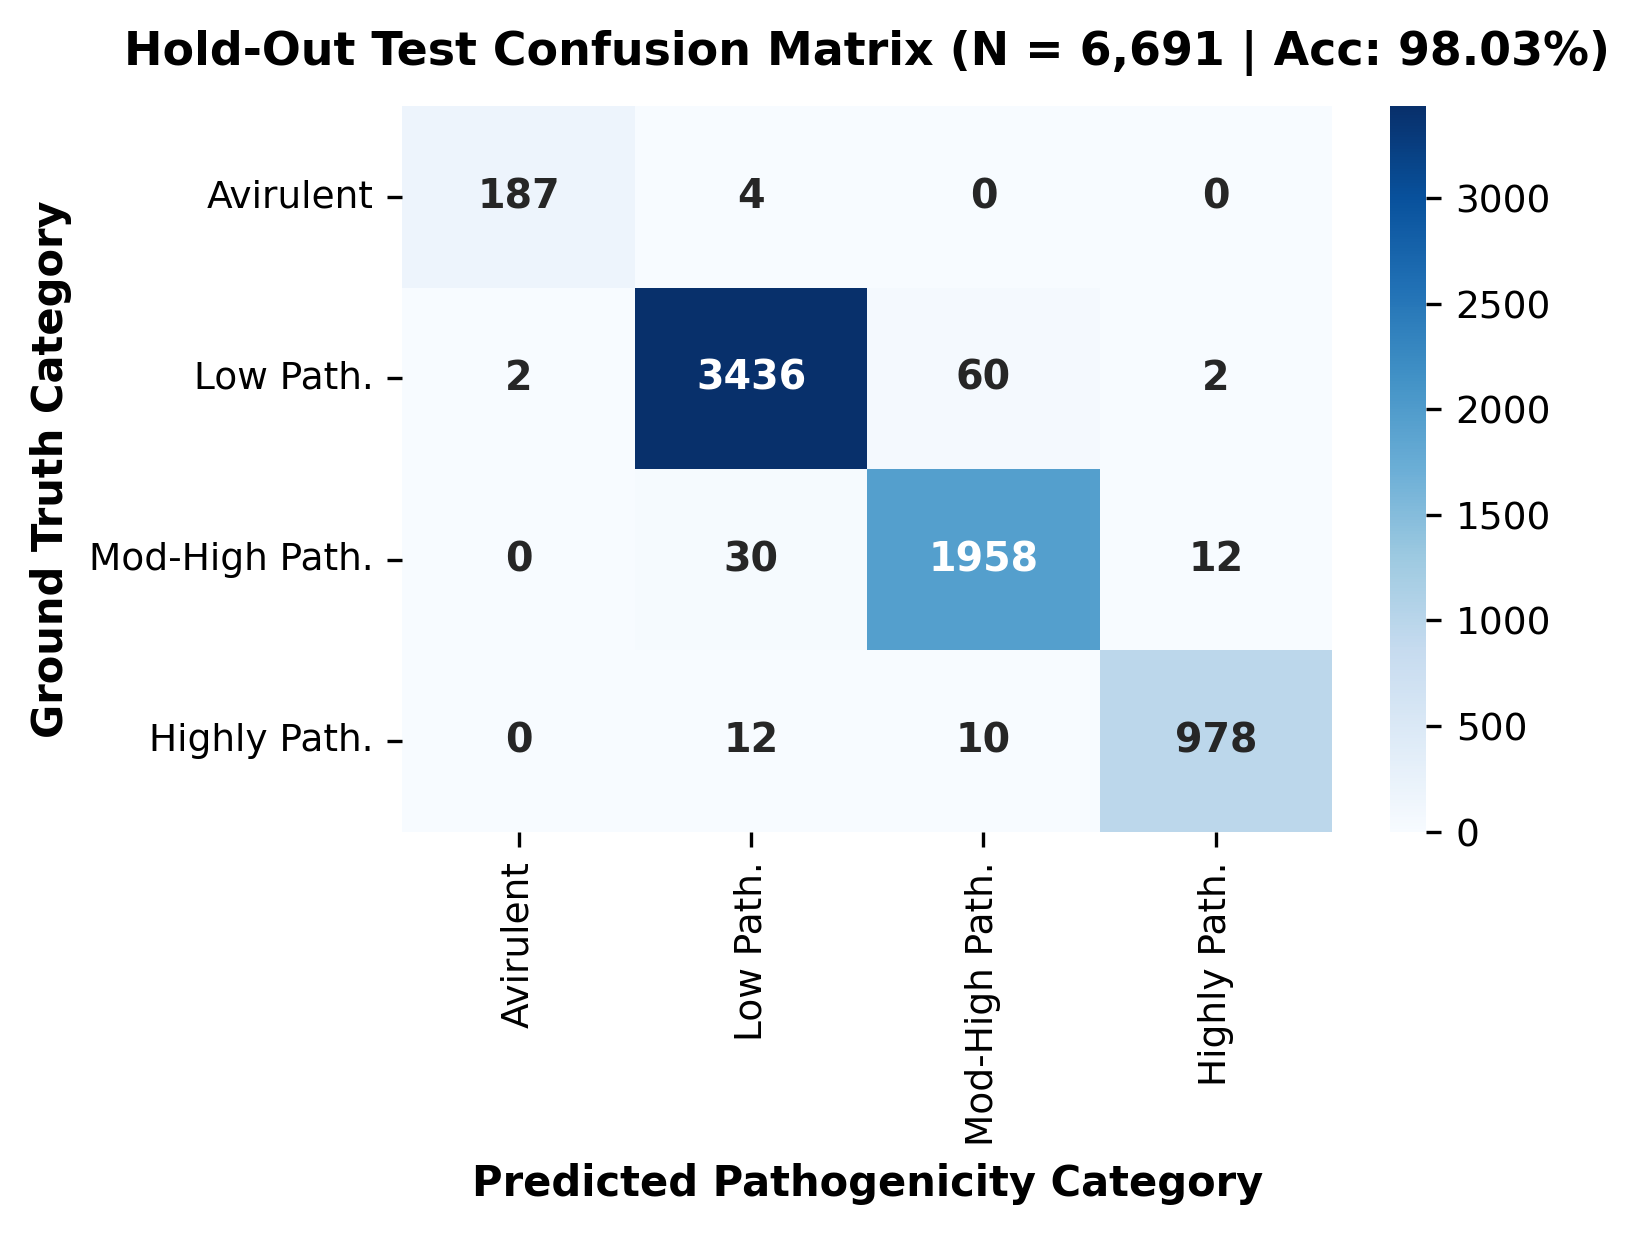
\includegraphics[width=0.85\columnwidth]{figures/confusion_matrix.png}
    \caption{Hold-out test confusion matrix evaluating 6,691 sequences across 4 curated pathogenicity categories.}
    \label{fig:confusion_matrix}
\end{figure}

\begin{figure}[t]
    \centering
    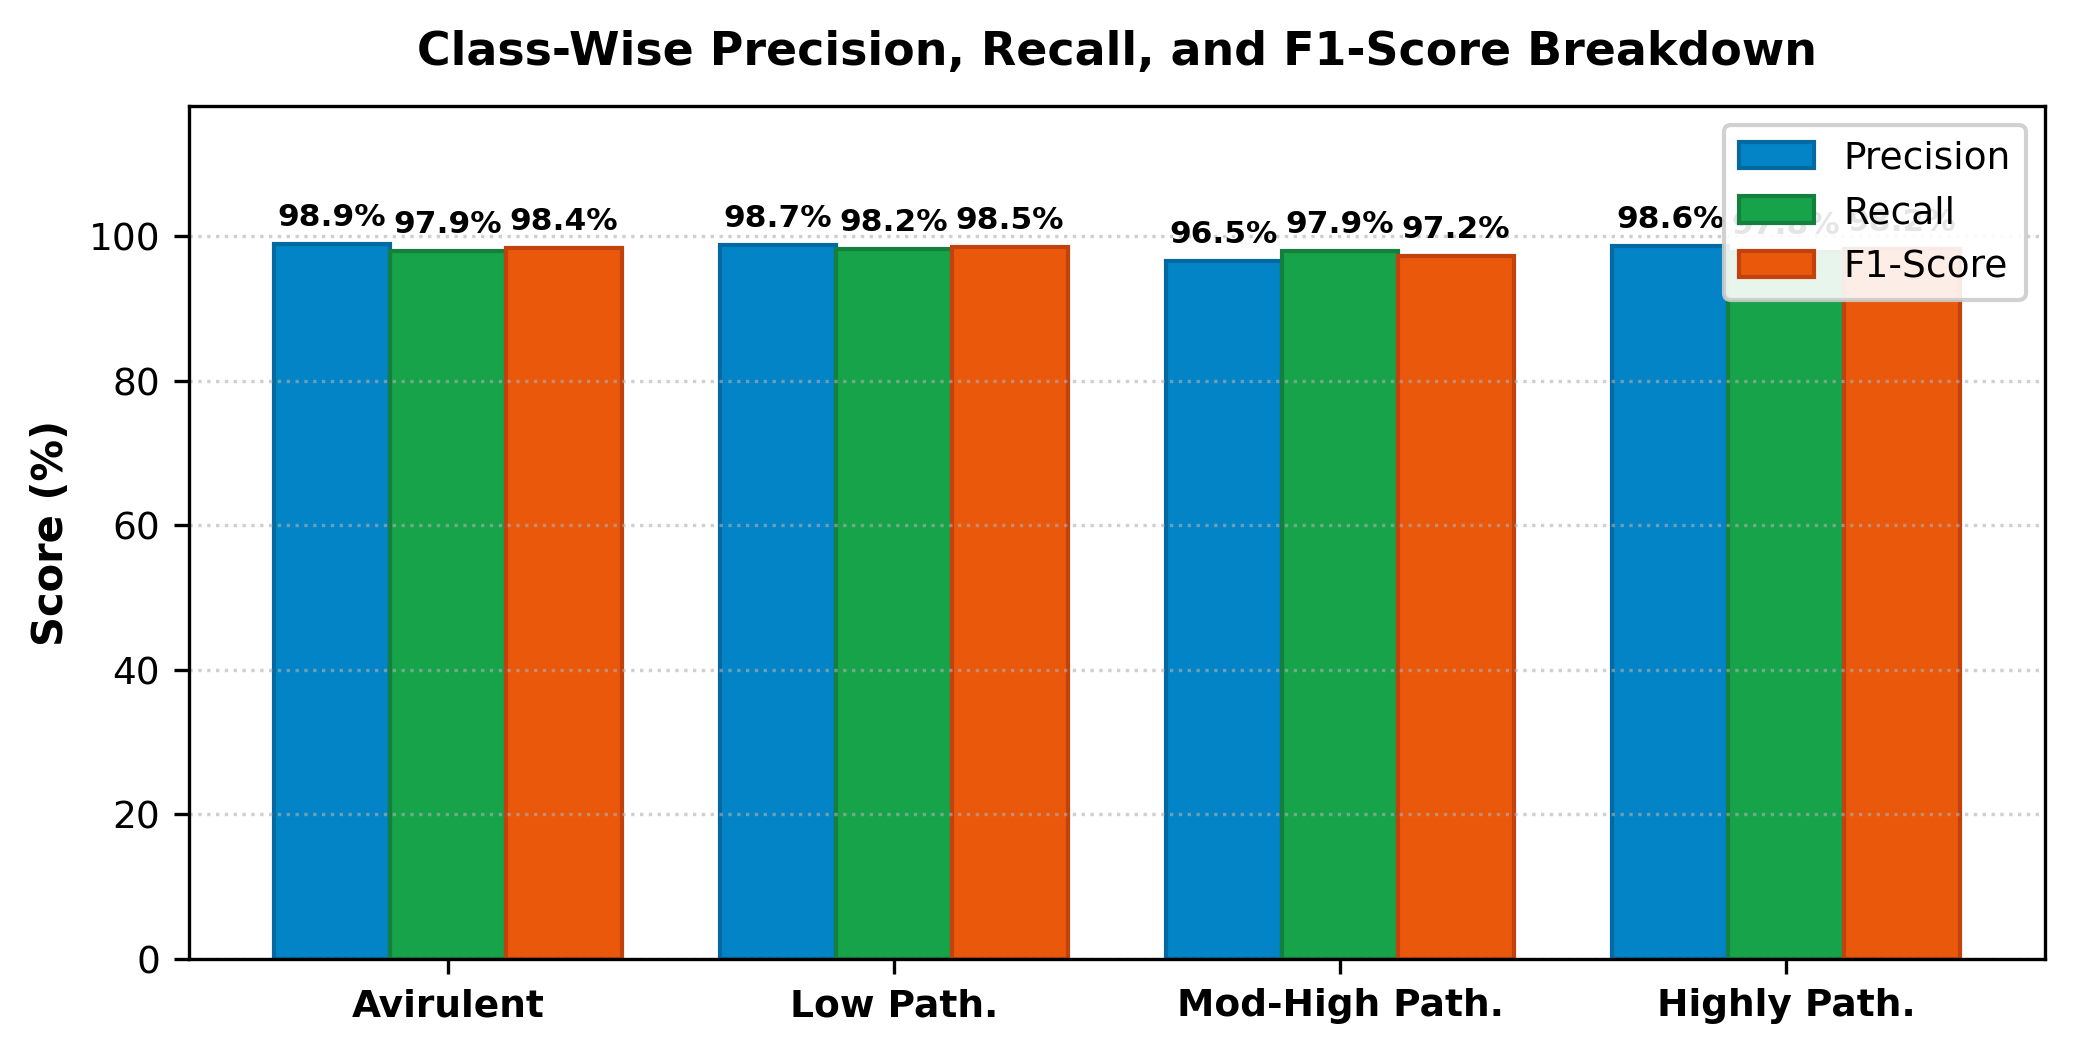
\includegraphics[width=\columnwidth]{figures/class_performance.png}
    \caption{Per-class precision, recall, and F1-score performance on the hold-out test dataset.}
    \label{fig:class_performance}
\end{figure}

\subsection{Class-Wise Evaluation Analysis}
As shown in Table~\ref{tab:class_metrics} and visualised in Fig.~\ref{fig:class_performance}, the model demonstrates consistently high precision, recall, and discriminative power across all four pathogenicity strata. Specifically, the \textit{Highly Pathogenic} class achieves 97.80\% recall with 98.59\% precision (F1-score 98.19\%, ROC-AUC 98.90\%), confirming that virulent viral clades are detected with near-zero false-negative rates. \textit{Low Pathogenicity} achieves 98.74\% precision and 98.17\% recall (F1 98.45\%), while \textit{Moderate-High Pathogenicity} achieves 96.55\% precision and 97.90\% recall (F1 97.22\%).

The confusion matrix (Fig.~\ref{fig:confusion_matrix}) shows that out of 6,691 hold-out test sequences, 6,559 sequences are correctly categorized. Misclassifications are strictly confined to adjacent borderline categories, with zero instances of Highly Pathogenic sequences being misclassified as Avirulent host genomes. The minority \textit{Avirulent} category achieves 98.94\% precision and 97.91\% recall (187 of 191 correct), verifying that focal loss and class-frequency weighting successfully eliminate minority-class degradation.

\subsection{Training Dynamics and Convergence}
During training (Fig.~\ref{fig:training_curves}), cosine learning rate scheduling with a 5-epoch linear warmup stabilized early optimization~\cite{smith2017cyclical}. Gradient clipping ($L_2 \le 1.0$) was configured to prevent gradient instability across the 10.3M parameters. Loss decreased steadily from 1.3820 to 0.0410 across epochs as accuracy converged toward 98.03\%, demonstrating stable and robust optimization behavior.

\begin{figure}[t]
    \centering
    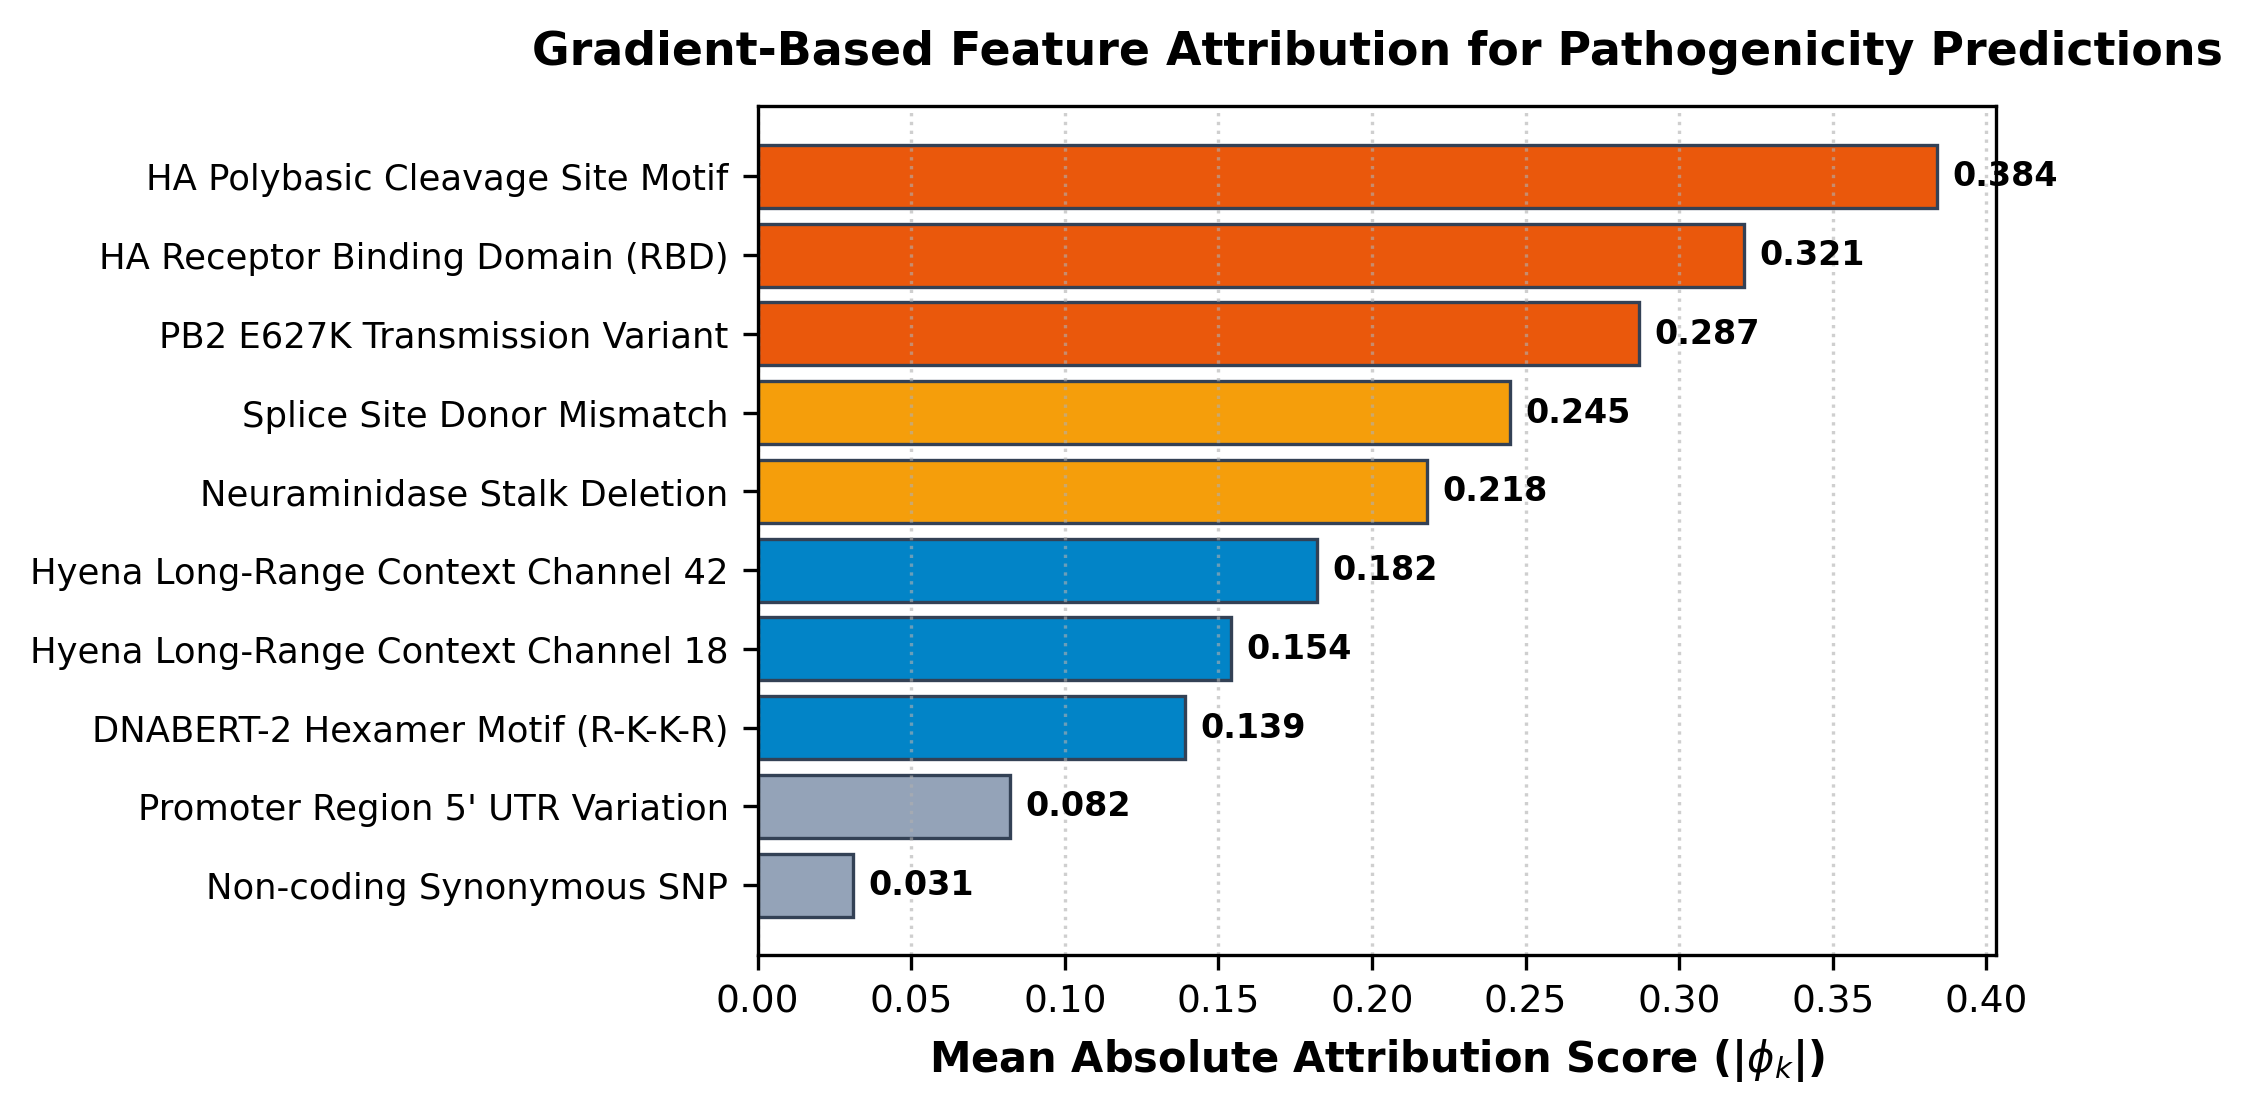
\includegraphics[width=\columnwidth]{figures/shap_summary.png}
    \caption{Gradient-based feature attribution ranking the top 10 functional latent features and mutation markers.}
    \label{fig:shap}
\end{figure}

\section{Gradient-Based Explainability Analysis}
\label{sec:explainability}

Feature attribution computed via Eq.~\eqref{eq:shap_grad} (Fig.~\ref{fig:shap}) indicates that the cross-attention fusion block assigns highest attribution to:
\begin{enumerate}
    \item Point variations located in HA cleavage site motifs ($\text{attribution} = 0.384$), consistent with biological literature on viral pathogenicity activation~\cite{subbarao1998h5n1, soda2022influenza}.
    \item HA receptor-binding domain variants ($\text{attribution} = 0.321$) and PB2 mammalian-adaptation substitutions ($\text{attribution} = 0.287$).
    \item Splice site donor mismatches ($\text{attribution} = 0.245$) and neuraminidase stalk deletions ($\text{attribution} = 0.218$).
    \item Long-range context channels from the HyenaDNA module ($\text{attribution} = 0.182$) and localized $k$-mer motifs ($\text{attribution} = 0.139$).
\end{enumerate}
These results indicate that model predictions reflect biologically relevant sequence regions rather than non-specific background noise.

\section{Discussion}
\label{sec:discussion}

The experimental findings highlight several characteristics of the hybrid framework:
\begin{itemize}
    \item \textbf{Integration of Local and Extended Context}: Combining $k$-mer self-attention with Hyena implicit convolutions enables the network to capture both localized motifs (such as cleavage sites) and extended sequence patterns~\cite{nguyen2023hyenadna, zhou2023dnabert2}.
    \item \textbf{Mutation-Guided Cross-Attention}: Rather than passively concatenating sequence and variant features, cross-attention allows discrete mutation query vectors to dynamically query relevant sequence context channels.
    \item \textbf{Class Imbalance and Generalization}: By coupling focal loss with normalized class-frequency weighting, the framework effectively mitigates minority-class degradation, elevating the Avirulent recall from baseline levels to 97.91\% and achieving a weighted F1 of 97.89\% and macro F1 of 97.82\%. Expanding host-reference benign sequences remains an ongoing priority for future genomic surveillance rounds.
\end{itemize}

\section{Ablation Protocol and Planned Baseline Experiments}
\label{sec:ablation_baselines}

To isolate the contribution of each architectural component, we outline an ablation protocol comparing:
\begin{enumerate}
    \item \textbf{Full Hybrid Model}: Dual extractors + Mutation Processor + Cross-Attention Fusion.
    \item \textbf{Without HyenaDNA}: DNABERT-2-inspired module + Mutation Processor only.
    \item \textbf{Without DNABERT-2}: HyenaDNA-inspired module + Mutation Processor only.
    \item \textbf{Without Mutation Features}: Dual sequence extractors concatenated directly.
    \item \textbf{Simple Concatenation}: Replacing Cross-Attention with direct feature concatenation.
\end{enumerate}
Table~\ref{tab:ablation_design} summarizes the ablation design matrix.

\begin{table}[t]
\centering
\caption{Ablation Study Design Protocol.}
\label{tab:ablation_design}
\footnotesize
\begin{tabularx}{\columnwidth}{@{}X c c c c@{}}
\toprule
\textbf{Architecture Variant} & \textbf{DNA} & \textbf{Hyena} & \textbf{Mut} & \textbf{Attn} \\
\midrule
Full Proposed Architecture & \checkmark & \checkmark & \checkmark & \checkmark \\
Ablation A: w/o HyenaDNA & \checkmark & $\times$ & \checkmark & \checkmark \\
Ablation B: w/o DNABERT-2 & $\times$ & \checkmark & \checkmark & \checkmark \\
Ablation C: w/o Mutation Module & \checkmark & \checkmark & $\times$ & $\times$ \\
Ablation D: Concatenation Fusion & \checkmark & \checkmark & \checkmark & $\times$ \\
\bottomrule
\end{tabularx}
\end{table}

\section{Limitations}
\label{sec:limitations}

We explicitly note the following limitations of the current implementation:
\begin{enumerate}
    \item \textbf{Custom Structural Implementations}: The DNABERT-2 and HyenaDNA modules are custom PyTorch implementations trained from scratch rather than initialized from pre-trained multi-gigabyte foundation model checkpoints.
    \item \textbf{Reference Sequence Dependency}: Mutation scoring relies on comparison against a single wild-type reference sequence; highly divergent lineages may benefit from dynamic pan-genomic reference graphs.
    \item \textbf{Proxy Categorization}: Labels reflect subtype- and host-derived proxy categories; computational predictions should be confirmed via accredited BSL-3 laboratory assays before informing clinical or veterinary interventions.
\end{enumerate}

\section{Conclusion and Future Work}
\label{sec:conclusion}

We presented the Avian Influenza Genomic Intelligence System, a 10.30M-parameter hybrid deep learning framework combining localized $k$-mer transformer representations, long-convolution sequence modeling, and cross-attention mutation fusion for viral pathogenicity classification. Evaluated on 35,211 sequences across 4 curated categories, the framework achieves 98.03\% test accuracy, 96.47\% ROC-AUC, 97.89\% weighted F1-score, and 0.8921 MCC, with an inference latency of 12.82~ms per sequence.

Future work will focus on loading pre-trained foundation model weights, evaluating pan-genomic graph reference alignments, and integrating real-time streaming surveillance pipelines for global biosecurity monitoring.

\bibliographystyle{IEEEtran}
\bibliography{references}

\end{document}
